%
%% Please do not remove author note!
%%%
%%%% Created by Kacper B Sokol (k.sokol.2011 [at] my.bristol.ac.uk)
%%%
%% Please do not remove author note!
%

\documentclass[11pt, letterpaper]{article}            % report | leqno, pdflatex

% \usepackage[]{algorithm2e}
% \usepackage[usenames,dvipsnames]{color}
% \usepackage[letterspace=3pt]{microtype} % linespacing

\usepackage[left=3.17cm, right=3.17cm, bottom=2.54cm, top=2.54cm]{geometry}
\usepackage{graphicx}                                                 % graphics
\usepackage{color}                                              % custom colours
\usepackage{lipsum}                                        % just a space filler
\usepackage{soul}												% letter spacing
\definecolor{natc}    {RGB}{021,055,090}
\definecolor{subc}    {RGB}{121,121,121}
\definecolor{headc}   {RGB}{034,065,094}
\definecolor{headerc} {RGB}{127,145,173}
\definecolor{footerc} {RGB}{128,128,128}
\definecolor{footerc1}{RGB}{192,192,192}
\definecolor{linec}   {RGB}{237,237,237}
\usepackage[absolute]{textpos}      % absolute positioning of images | showboxes
\usepackage{cite}                                                        % BiTeX
\usepackage[square]{natbib}									  % Harvard citation

\usepackage{datetime}                                              % custom date
\newdateformat{motd}{\monthname[\THEMONTH] \THEYEAR}               % custom date

\usepackage{fontspec}                                      % all different fonts
\usepackage{xcolor}
\usepackage{titlesec}
\defaultfontfeatures{Ligatures=TeX}
\setsansfont{Arial}
\setmainfont{Times New Roman}
\titleformat*{\section}{\fontsize{16}{18}\color{headc}\bfseries\sffamily}
\titleformat*{\subsection}{\fontsize{13}{15}\color{headc}\bfseries\sffamily}
\titleformat*{\subsubsection}{\fontsize{11}{13}\color{headc}\bfseries\sffamily}
\newfontfamily\headerfont[Ligatures=TeX]{Calibri}
\newfontfamily\footerfont[Ligatures=TeX]{Times New Roman}


\usepackage[linktocpage=true]{hyperref}						    % click-able ToC
\usepackage{tocloft}
\renewcommand{\contentsname}							   % ...
	{\fontsize{16}{18}\color{headc}\bfseries\sffamily	   % ...
	Table of Contents}									   % change name for ToC

\setcounter{tocdepth}{3}
\cftsetindents{section}{0.0em}{1.0em}
\cftsetindents{subsection}{1.0em}{2.0em}
\cftsetindents{subsubsection}{2.0em}{3.0em}
% \cftsetindents{paragraph}{0.5in}{0.5in}
% \makeatletter \renewcommand*\l@section{\@dottedtocline{1}{1.5em}{2.3em}} \makeatother
\makeatletter \renewcommand*\l@section{\@dottedtocline{0}{0.0em}{1.5em}} \makeatother
% \renewcommand{\cftsecfont}{\fontsize{19}{13}\color{headc}\bfseries\sffamily}


% define headers and footers
\usepackage{etoolbox,fancyhdr,xcolor}
\pagestyle{fancy}
\newcommand{\footrulecolor}[1]{\patchcmd{\footrule}{\hrule}{\color{#1}\hrule}{}{}} % footer colour
\fancyhead{} % clear all header fields
\renewcommand{\headrulewidth}{0pt} % no line in header area
\fancyhead[LE,LO]{\headerfont\fontsize{9}{11}\selectfont\color{headerc}\textbf{CERN openlab Summer Student Report}}
\fancyhead[RE,RO]{\headerfont\fontsize{9}{11}\selectfont\color{headerc}\textbf{\the\year}}
\fancyfoot{} % clear all footer fields

%%%%%%%%%%%%%%%%%%%%%%%%%%%%%%%%%%%%%%%%%%%%%%%%%%%%%%%%%%%%%%%%%%%%%%%%%%%%%%%%
%%%%%%%%%%%%%%%%%%%%%%%%%%%%%%%%%%%%%%%%%%%%%%%%%%%%%%%%%%%%%%%%%%%%%%%%%%%%%%%%
%%%%%%%%%%%%%%%%%%%%%%%%%%%%%%%%%%%%%%%%%%%%%%%%%%%%%%%%%%%%%%%%%%%%%%%%%%%%%%%%
%%%%%%%%%%%%%%%%%%%%%%%%%%%%%%%%%%%%%%%%%%%%%%%%%%%%%%%%%%%%%%%%%%%%%%%%%%%%%%%%
%%%%%%%%%%%%%%%%%%%%%%%%%%%%%%%%%%%%%%%%%%%%%%%%%%%%%%%%%%%%%%%%%%%%%%%%%%%%%%%%
%%%%%%%%%%%%%%%%%%%%%%%%%%%%%%%%%%%%%%%%%%%%%%%%%%%%%%%%%%%%%%%%%%%%%%%%%%%%%%%%
\usepackage[]{algorithm2e}
\usepackage{amsmath}
\usepackage{amsfonts}    % fancy maths font
\usepackage{mathrsfs}    % fancy maths font
\usepackage{dsfont}      % indocator finction
\usepackage{mathtools}
%%%%%%%%%%%%%%%%%%%%%%%%%%%%%%%%%%%%%%%%%%%%%%%%%%%%%%%%%%%%%%%%%%%%%%%%%%%%%%%%

\begin{document}

\begin{textblock*}{0mm}(-12.2mm,-0.3mm)\noindent \includegraphics*{./gfx/bg.png}\end{textblock*}
\begin{textblock*}{0mm}(144.3mm,238.3mm)\noindent \includegraphics*{./gfx/openlab.png}\end{textblock*}
\begin{textblock*}{150mm}(114.2mm,140.0mm)\noindent
\parbox{8cm}{\bfseries\sffamily\textbf{\fontsize{20}{20}\selectfont\color{natc}Making sense of data streams:}}\\[.3em]
\parbox{8cm}{\bfseries\sffamily\textbf{\fontsize{20}{20}\selectfont\color{natc}Complex Event Processing for Controls Applications}}\\[36pt]
{\bfseries\sffamily\textbf{\fontsize{16}{20}\selectfont\color{natc}\motd\today}}\\[18pt]
{\sffamily\fontsize{14}{20}\selectfont\color{subc}Author:}\\
{\sffamily\fontsize{14}{20}\selectfont\color{subc}Kacper B.\ Sokol}\\[18pt]
{\sffamily\fontsize{14}{20}\selectfont\color{subc}Supervisor(s):}\\
{\sffamily\fontsize{14}{20}\selectfont\color{subc}Filippo Tilaro}\\
{\sffamily\fontsize{14}{20}\selectfont\color{subc}Axel Voitier}\\[18pt]
\textbf{\bfseries\sffamily\fontsize{11}{20}\selectfont\color{subc}CERN openlab Summer Student Report 2014}

\end{textblock*}
~
\thispagestyle{empty}\newpage

\section*{Project Specification}
CERN is currently investigating the usage of data analysis technologies to study the behavior of the industrial control systems. An activity related to these analysis is using Complex Event Processing tools to classify a real abnormal behavior from one generated by a human intervention on the system. This CEP classification will run over textual logs mainly. A list of events to match will be given as input. The selected CEP tools will be either Drools or \texttt{Esper}. The work will consist of installing one of these tools and develop the classification system with it.
\newpage

\section*{Abstract}
This project aims at build a tool to process live stream of data generated by various sensors. The program uses \texttt{Esper} package to receive data feeds, apply user defined rules, and pass resulting information to clustering framework.\\
The last step employs \emph{Affinity Propagation} based clustering algorithm, which choice is motivated by no need of defining number of clusters prior to program initialisation, and documented overall good performance in live analysis cases.\\
Our approach is then compared on against static clustering algorithm, and in-depth results analysis follows.
\newpage

{\fontsize{11}{13}\sffamily\linespread{1.750}\selectfont\tableofcontents}
\thispagestyle{fancy}\newpage

% Start footer here
\fancyfoot{} % clear all footer fields
\renewcommand{\footrulewidth}{0.4pt} % no line in header area
\footrulecolor{linec}
\fancyfoot[LE,LO]{\footerfont\fontsize{9}{11}\selectfont \textcolor{footerc}{\textbf{\thepage~$|$}}~\textcolor{footerc1}{\footerfont\so{\texttt{Page}}}} % \fontfamily{ppl}\selectfont

\section{Introduction}
In machine learning, unsupervised clustering aims at discovering cluster structure underpinning the data. There are many state-of-the-art algorithms designed to solve this problem performing well on the data. All major algorithms deal with static data, forcing user to define many parameter prior to classification. The example of this might be predefined number of clusters. Also, many of this algorithm need static distribution of data, and what is more static data.\\
The major trial to address this issue was presented by~\citep{zhang2013data} with clustering algorithm based on affinity propagation that adressess all of the above concerns: adapts the number of clusters to the data therefere handles unstationary data distribution, and what is more works on a data stream.\\
I aim at extending presented above approach with \texttt{Esper} framework. I add possibility of modular feature extractors with all advantages of time windowing the signal stream.\\
I provide complete feature extraction system based on \texttt{EPL} statement and clustering solution, capable of clustering live stream of data whit chosen by user complex features.\\



\subsection{What is \emph{Complex Event Processing}}
\emph{Complex Event Processing} is a software family facilitating high throughput, complex analysis of live data feeds.\\
The concept behind it is similar to database querying, but doing it on live data. It gives possibility of applying filters, functions, and statistical analysis to chosen part of signal by \emph{querying} the signal.

\subsection{What is \texttt{Esper}}
\texttt{Esper} tool used to handle incoming data streams and to extract chosen features belongs to family of \emph{Complex Event Processing} tools. These software analyses multiple live data streams. Its main advantage is \emph{time windowing}, which allows to focus on a specific time period. Aforementioned feature can work in multiple modes:
\begin{description}
	\item[Time] incoming data from last $t$ milliseconds/seconds/minutes/etc.\ are processed.
	\item[Time batch] data are processed in $t$ milliseconds/seconds/minutes/etc.\ batches i.e.\ algorithm collects data for $t$ units of time, then process them and repeat this cycle.
	\item[Length] $n$ latest events are processed.
\end{description}
The package also allow joining multiple incoming signals for processing purposes. With proprietary \texttt{EPL} querying language the analysis boils down to simple statements. One approach is to hard-code the EPL queries but it is also possible to provide them as module(text file) what gives flexibility of new extracting features without need of stopping the analysis.\\
\texttt{Esper} is available as \texttt{Java} and \texttt{.NET} framework hence is multi-platform and easy to incorporate. It can also work as server with possibility of introducing on-the-go changes via AIP like rules can injection on the fly.\\

\subsection{Why to use it}
The major advantage of \texttt{Esper} is ability of processing millions of events per second, low computational complexity, and no time consuming read-write disk processes.\\
The data processing can be describe in ``\textbf{4D}'' steps:
\begin{description}
\item[\textit{D}etect] events of interest.
\item [\textit{D}erive] events complying with specified rules.
\item [\textit{D}ecide] what to do based on gathered evidences(data).
\item [\textit{D}o] the action bonded with occurring event.
\end{description}

\subsubsection{CEP at CERN}
I adopt the ``\textbf{4D}'' flow by: \emph{detecting} incoming signals from the sensors(generators); \emph{deriving} the specified features from the signal; \emph{deciding} to send the features to clustering algorithm; and \emph{do}ing the classification.

\subsection{Applications}
The software is mainly used in high throughput analysis services, where analysis must be easily adaptable (rules injection). The following examples show different aspects of \emph{Complex Event Processing} tools being used.
\subsubsection{Nuclear Power Plant}
While managing nuclear plant there is plenty of factors that may lead to disaster:
\begin{itemize}
\item core temperature,
\item cooling pumps status,
\item seismic movements,
\item weather forecast,
\item electricity usage projections.
\end{itemize}
Only specific state of each of this factors should raise the alarm.
\subsubsection{Stock market}
In this example we consider signals as all the real time price processes. We filter them with EPL statements, and .


\section{Model of processing}
Describe the overview of model of processing given in below figure\\
\begin{figure}[htbp]
	\centering
	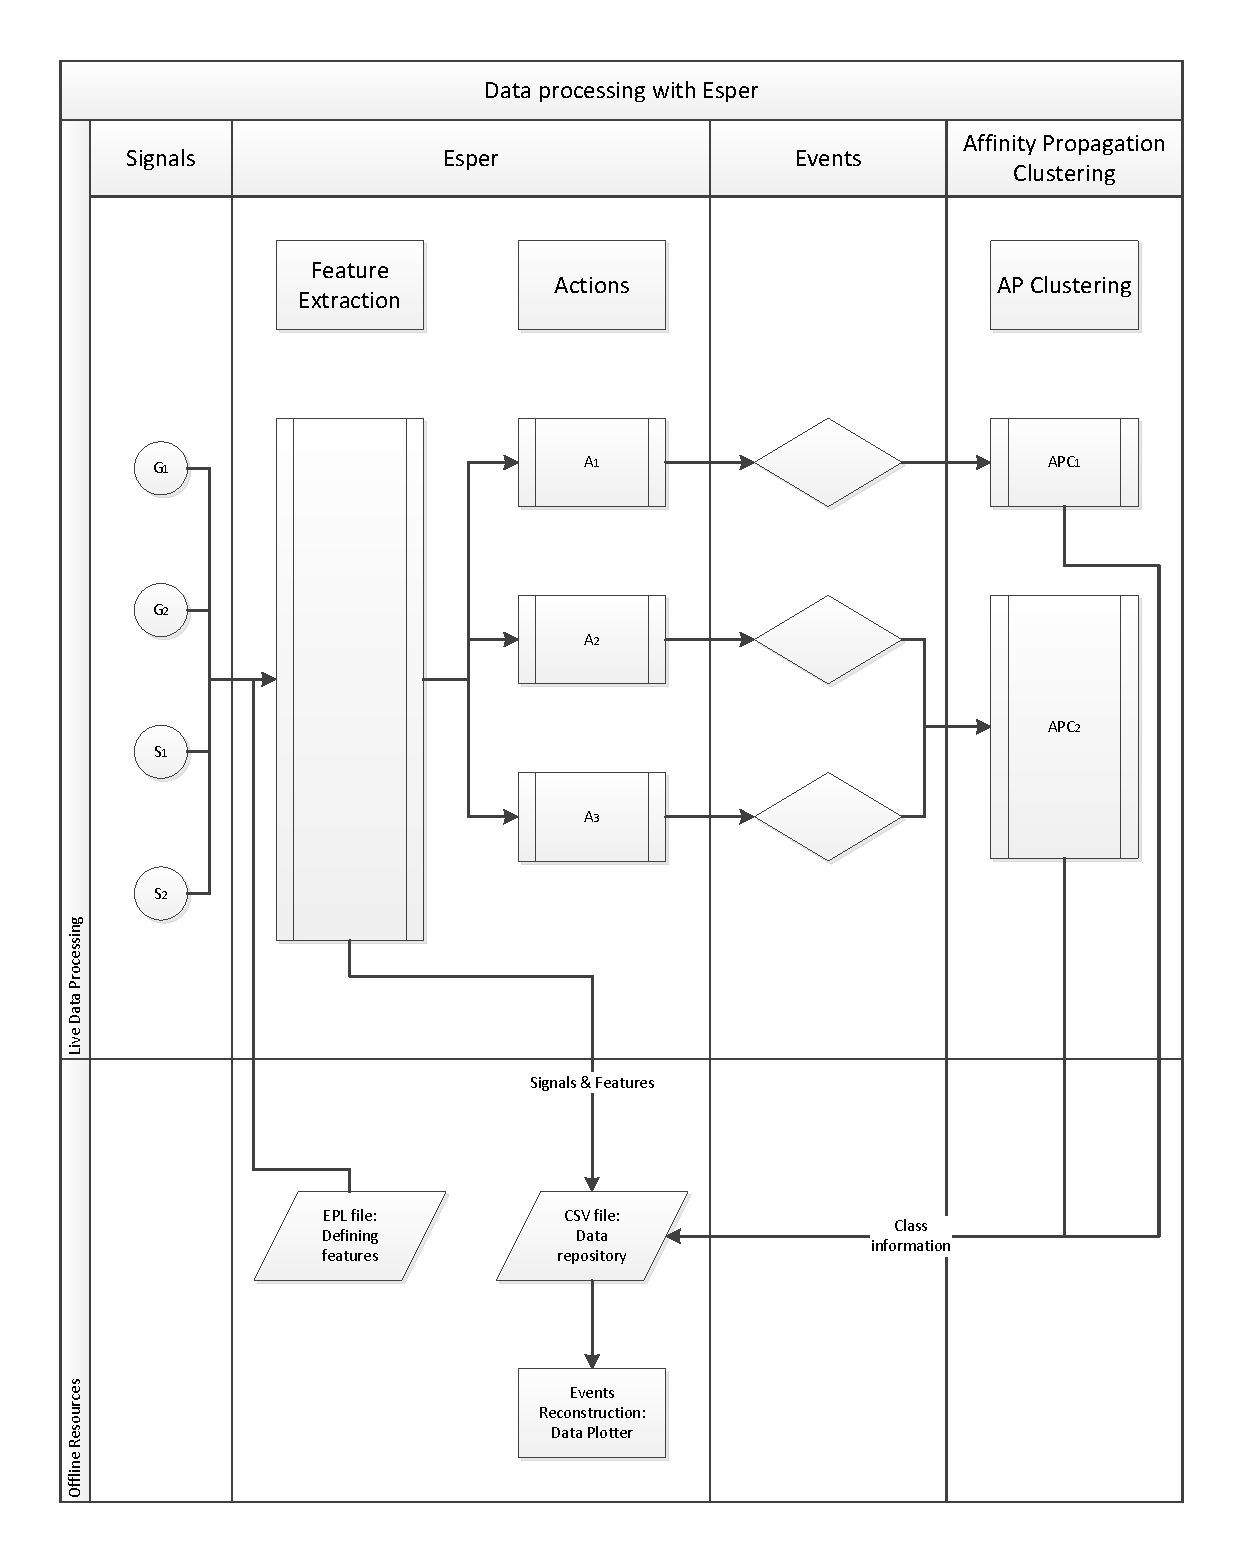
\includegraphics[width=\textwidth]{./gfx/model.pdf}
  \caption{Data processing model.\label{fig:model}}
\end{figure}
and all the components\\

\subsection{\texttt{Esper} engine}
describe the engine\\

\subsection{Generators / signals}
gens, \\

\subsection{Rules---Feature extraction}
give file with rules here
Rules -> feature extractors\\

\subsection{Listeners for change}
Engine Listeners\\

\subsection{Clustering with Affinity Propagation}
Clustering model~\citep{zhang2013data}\\
\begin{figure}[htbp]
	\centering
	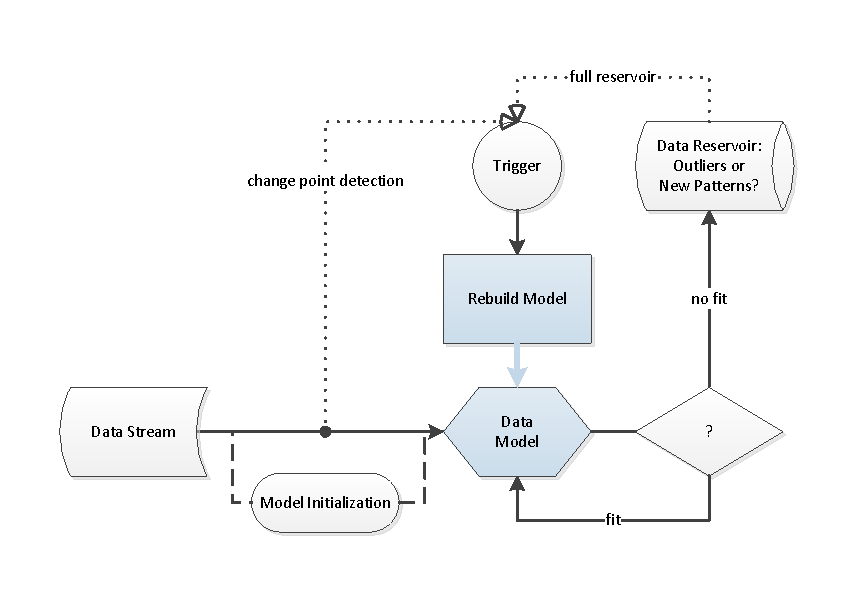
\includegraphics[width=\textwidth]{./gfx/APC.pdf}
  \caption{Stream clustering model.\label{fig:APC}}
\end{figure}

\RestyleAlgo{boxed}
\SetAlCapSkip{1em}
\LinesNumbered
\vspace{2cm}
\begin{algorithm}[h]
  \KwData{Posterior distributions for each action---$\left\{ 
p_a(\cdot|\mathscr{L}_t,x_t) : a \in \mathscr{A} \right\}$}
  \For{$a \in \mathscr{A}$}{
    \text{sample: }$\mathscr{Q}^\text{Th}_{t,a} \leftarrow 
p_a(\cdot|\mathscr{L}_t,x_t)$ \;
  }
  sample $a_t$ uniformly from $\operatorname{arg\,max}_{a \in \mathscr{A}} 
\mathscr{Q}^\text{Th}_{t,a}$ \;
 \caption{Affinity Propagation Clustering.\label{alg:APC}}
\end{algorithm}
\vspace{2cm}

\subsection{Data visualization}
describe python script to vizualise the data\\


\section{Results and comparison}
Describe results of AP clustering

\subsection{why particulat algorithms were chosen}
\subsection{WEKA algorithms review}

\section{Lookahead}
what can be improved in the programm\\
nice features to add\\

\section{Conclusions}
What is working\\
how is it helpful



\begin{center} \noindent \line(1,0){250} \end{center}	    % Optional ending line


%% Start References (a.k.a. bibliography)
\newpage								 								 % Optional new page before Bibliography
\bibliography{bibliography.bib}{}
\bibliographystyle{plainnat}

\end{document}
